\documentclass[nooutcomes]{ximera}
%% handout
%% space
%% newpage
%% numbers
%% nooutcomes

%I added the commands here so that I would't have to keep looking them up
%\newcommand{\RR}{\mathbb R}
%\renewcommand{\d}{\,d}
%\newcommand{\dd}[2][]{\frac{d #1}{d #2}}
%\renewcommand{\l}{\ell}
%\newcommand{\ddx}{\frac{d}{dx}}
%\everymath{\displaystyle}
%\newcommand{\dfn}{\textbf}
%\newcommand{\eval}[1]{\bigg[ #1 \bigg]}

%\begin{image}
%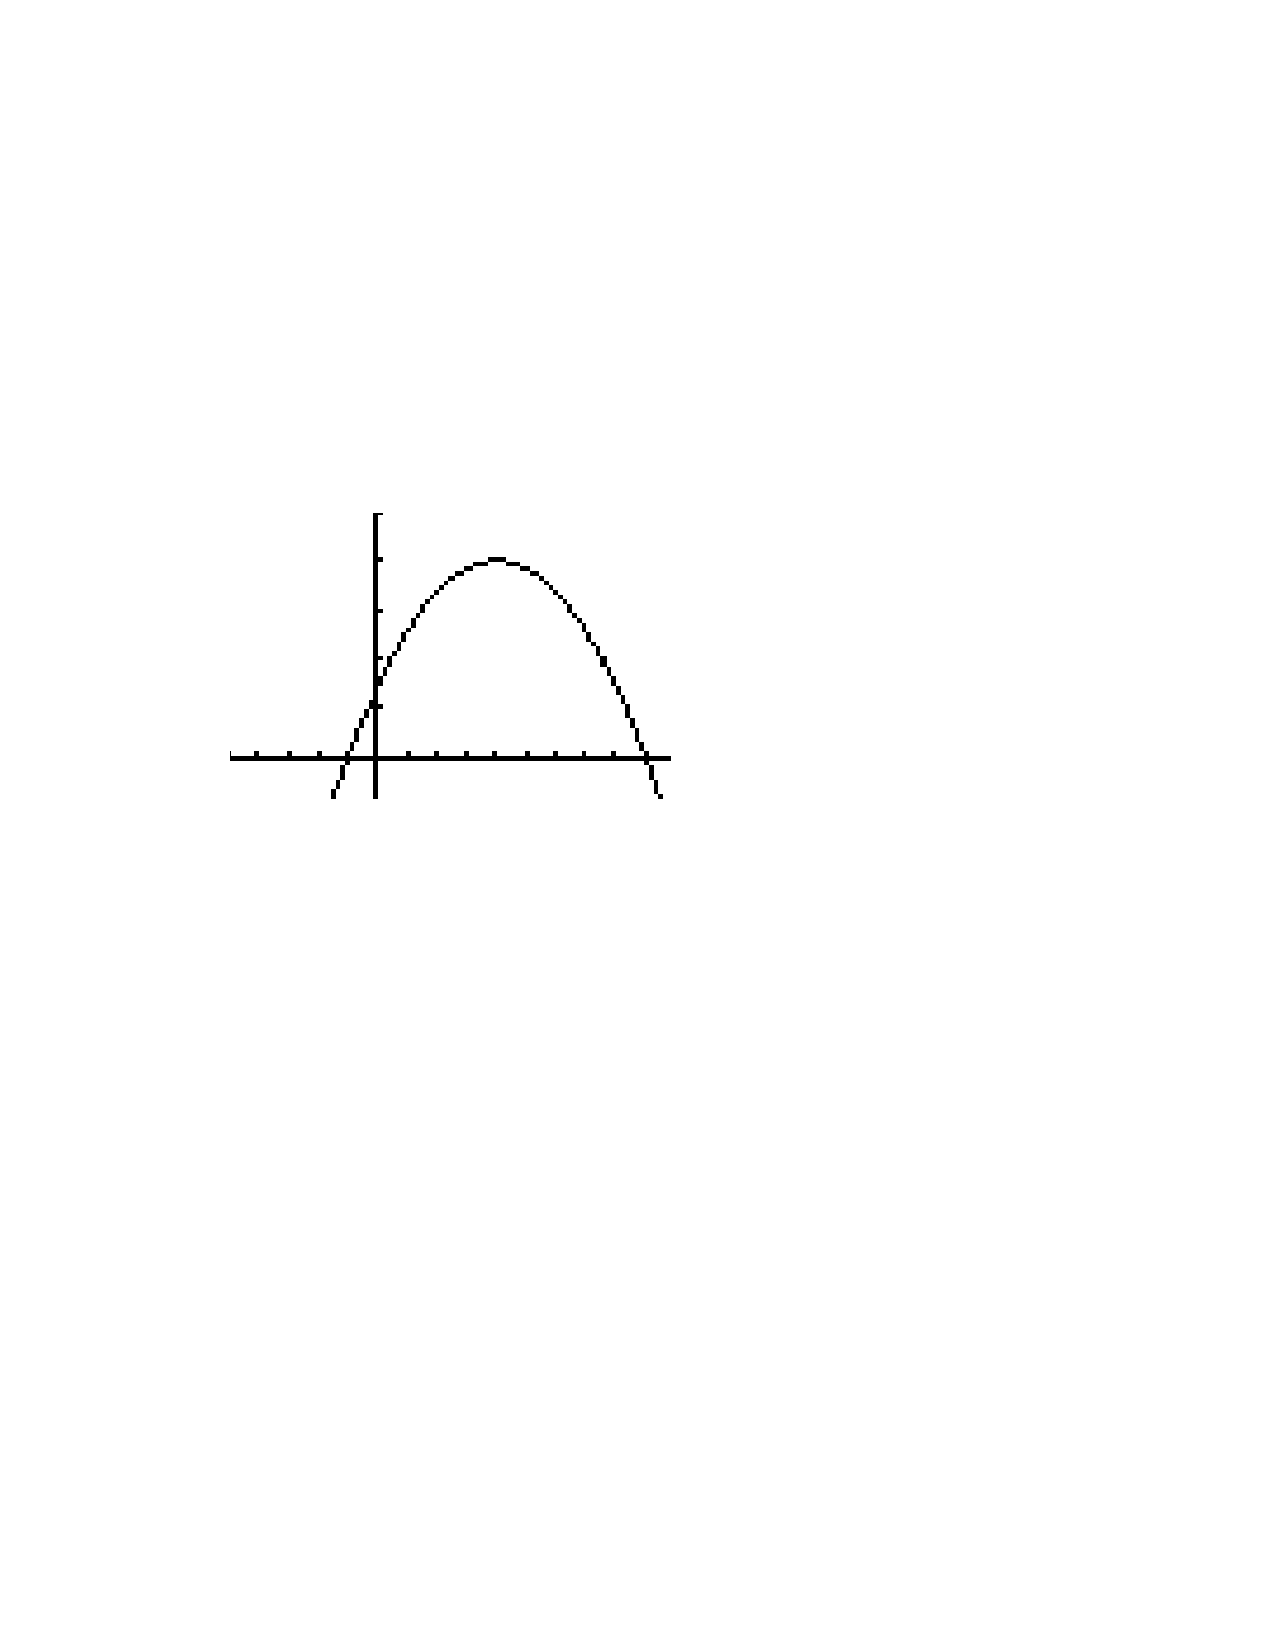
\includegraphics[trim= 170 420 250 180]{Figure1.pdf}
%\end{image}


\newcommand{\RR}{\mathbb R}
\renewcommand{\d}{\,d}
\newcommand{\dd}[2][]{\frac{d #1}{d #2}}
\renewcommand{\l}{\ell}
\newcommand{\ddx}{\frac{d}{dx}}
\newcommand{\dfn}{\textbf}
\newcommand{\eval}[1]{\bigg[ #1 \bigg]}

\usepackage{multicol}

\renewenvironment{freeResponse}{
\ifhandout\setbox0\vbox\bgroup\else
\begin{trivlist}\item[\hskip \labelsep\bfseries Solution:\hspace{2ex}]
\fi}
{\ifhandout\egroup\else
\end{trivlist}
\fi} %% we can turn off input when making a master document

\title{3.10 Derivatives of Inverse Trig Functions (Solutions)}  

\begin{document}
\begin{abstract}		\end{abstract}
\maketitle

\section{Warm up:} 
Explain what each of the following means:
	\begin{enumerate}
	
	%part a
	\item  $\sin^{-1}(x)$
		\begin{freeResponse}
		This denotes the inverse function to $sin(x)$, sometimes denoted by $\arcsin(x)$.  
		\end{freeResponse}	
		
	%part b
	\item  $\left( \sin(x) \right)^{-1}$
		\begin{freeResponse}
		This means $\sin(x)$ raised to the $-1$ power, i.e. $\frac{1}{\sin(x)}$.  
		\end{freeResponse}	
		
	%part c
	\item  $\sin \left(x^{-1} \right)$
		\begin{freeResponse}
		This means $\sin \left( \frac{1}{x} \right)$.
		\end{freeResponse}	
		
	%part d
	\item  $f^{-1}(x)$
		\begin{freeResponse}
		This denotes the inverse function of $f(x)$.  
		\end{freeResponse}	
		
	%part e
	\item  $f(x^{-1})$
		\begin{freeResponse}
		This means $f \left( \frac{1}{x} \right)$.
		\end{freeResponse}	
		
	%part f
	\item  $\left( f(x) \right)^{-1}$
		\begin{freeResponse}
		This means $f(x)$ raised to the $-1$ power, i.e. $\frac{1}{f(x)}$.  
		\end{freeResponse}	
	
	
		
	\end{enumerate}
		
		
		

	
	
	
	
	

\section{Group work:}



%problem 1
\begin{problem}
Find the derivatives of the following functions:
	\begin{enumerate}
	
	%part a
	\item  $f(x) = \sec^{-1} (\sqrt{x})$.
		\begin{freeResponse}
		$f'(x) = \frac{1}{\sqrt{x} \sqrt{x - 1}} \cdot \frac{1}{2} x^{-\frac{1}{2}} = \frac{1}{2x\sqrt{x-1}}$
		\end{freeResponse}
		
		
		
	%part b
	\item  $g(x) = \ln (\sin^{-1}(x))$.
		\begin{freeResponse}
		$g'(x) = \frac{1}{\sin^{-1}(x)} \cdot \frac{1}{\sqrt{1-x^2}}$.
		\end{freeResponse}
		
		
		
	%part c
	\item  $h(x) = \frac{1}{\tan^{-1}(x^2 + 4)}$.  
		\begin{freeResponse}
		$h'(x) = - \left( \tan^{-1}(x^2 + 4) \right)^{-2} \cdot \frac{1}{1 + (x^2 + 4)^2} \cdot (2x)$.
		\end{freeResponse}
		
		
		
	\end{enumerate}
		
		
\end{problem}
















%problem 2
\begin{problem}
Find the slope of the tangent line to the curve $y = f^{-1}(x)$ at $(4,7)$ if the slope of the tangent line to the curve $y=f(x)$ at $(7,4)$ is $\frac{2}{3}$.  
		\begin{freeResponse}
		Note that the statement ``the slope of the tangent line to the curve $y=f(x)$ at $(7,4)$ is $\frac{2}{3}$" specifically means that $f'(7) = \frac{2}{3}$.  The slope of the tangent line to the curve $y = f^{-1}(x)$ at $(4,7)$ is $(f^{-1})'(4)$, and so we use the formula for the derivative of the inverse function to compute:
		
		$(f^{-1})'(4) = \frac{1}{f'(7)} = \frac{1}{\frac{2}{3}} = \frac{3}{2}$.
		\end{freeResponse}
		
		
		

\end{problem}
	
	
	
	
	
	
	
	
			
			

%problem 3
\begin{problem}
Suppose that $f(x)$ is a differentiable function which is one-to-one.  Given the table of values below, find the value of $(f^{-1})'(7)$.  

\begin{tabular}{|c|c|c|c|}
\hline
\dfn{x}	&	1	&	7	&	11	\\
\hline
\dfn{f(x)}	&	7	&	11	&	1	\\
\hline
\dfn{f'(x)}	&	61	&	-17	&	71	\\
\hline
\end{tabular}

		\begin{freeResponse}
		$(f^{-1})'(7) = \frac{1}{f'(f^{-1}(7))}.$  Since $f(1) = 7$, $f^{-1}(7) = 1$.  Thus 
		$$(f^{-1})'(7) = \frac{1}{f'(1)} = \frac{1}{61}.$$
		\end{freeResponse}
		
		
		

\end{problem}











%problem 4
\begin{problem}
Find the derivative of $f^{-1}$ at the following points without solving for $f^{-1}$.
	\begin{enumerate}
	
	%part a
	\item  $f(x) = x^2 + 1$ (for $x \geq 0$) at the point $(5,2)$.  
		\begin{freeResponse}
		$(f^{-1})'(5) = \frac{1}{f'(2)}$.  Since $f'(x) = 2x$, $f'(2) = 4$.  Thus, $(f^{-1})'(5) = \frac{1}{4}$.  
		\end{freeResponse}
		
		
		
	%part b
	\item  $f(x) = x^2 - 2x - 3$ (for $x \leq 1$) at the point $(12, -3)$.  
		\begin{freeResponse}
		$(f^{-1})'(12) = \frac{1}{f'(-3)}$.  Since $f'(x) = 2x - 2$, $f'(-3) = -6 - 2 = -8$.  Thus, $(f^{-1})'(12) = - \frac{1}{8}$. 
		\end{freeResponse}
		
		
		
	\end{enumerate}
			
			
	
\end{problem}






	
	
	
	
	
	
	
	
	

	










								
				
				
	














\end{document} 


















